%!TEX TS-program = ../make.zsh

\newcommand\done{\checkmark\xspace}
\newcommand\inprogress{$\Rightarrow$\xspace}
\newcommand\tobedone{$\square$\xspace}

\section{Overview}
\subsection{Goal and Context}
\begin{frame}{Overview: Goal and Context}
  \begin{description}
    \item[Origin] \her{Diploma thesis} (2018-09) implementing direct photon propagation through hole ice in clsim in order to study hole-ice effects and improve understanding of low-energy systematics. \small \url{https://github.com/fiedl/hole-ice-study} \normalsize

    \item[Goal] \her{Bring} the new simulation \her{into} the icecube-simulation \her{framework} such that other icecubers can use it.

    \item[Context] \her{Service work} for the icecube collaboration in the beginning of my time as PhD student with icecube at ECAP/Erlangen.

    \item[Time frame] about 6 months
  \end{description}
\end{frame}

\subsection{Work to be done}
\begin{frame}{Overview: Work to be done}

  %\begin{itemize}
  %
  %
  %  \item[\done] Compile current icecube-simulation release V06-01-01 with Python 3 locally
  %  \item[\done] Make hole-ice code work with current icecube-simulation release V06-01-01
  %  \item[\inprogress] Provide example scripts for Python 3 (rather than Ruby)
  %  \item[\inprogress] Synchronize svn and git repositories of clsim
  %  \item[\tobedone] Re-implement ice tilt and ice anisotropy
  %  \item[\tobedone] Implement direct-detection switch
  %  \item[\tobedone] Merge hole-ice code into clsim trunk
  %\end{itemize}

  \setbeamertemplate{subsection in toc}{\hspace*{1em} \inserttocsubsection \vspace{2ex} \par}
  \tableofcontents[sectionstyle=hide,subsectionstyle=show,sections=2-]

  \bigskip \bigskip \small
  \done = done \ \ \ \inprogress = work in progress \ \ \ \tobedone\ = still to do
\end{frame}

\section{State of the individual steps}
\subsection{\done Compile IceSim V06-01-01 with Python 3}
\begin{frame}{\done Compile IceSim V06-01-01 with Python 3}
  \begin{itemize}
    \item In Stockholm (2018-09), the icecube software group requested the hole-ice example scripts to be provided in Python 3 (rather than Python 2 or Ruby) in order to push the migration to Python 3 forward.
    \item The current icecube documentation on how to install the framework still assumes Python 2: \url{http://software.icecube.wisc.edu/documentation/projects/cmake/supported_platforms/osx.html}
    \item[\done] Using Vagrant, a virtual-machine wrapper, I figured out a clean, reproducible way to install icecube-simulation V06-01-01 on macOS Sierra, which I use locally.
    \item[\done] Found a couple of issues and provided patches.
    \item[\tobedone] Still need to talk to the software group. Maybe they want to link or import the install  documentation.
  \end{itemize}

  \bigskip \her{Documented at: \url{https://github.com/fiedl/hole-ice-install}} \bigskip
\end{frame}

\subsection{\inprogress Port hole-ice code to clsim of icecube-simulation V06-01-01}
\begin{frame}{\inprogress Port hole-ice code to clsim of icecube-simulation V06-01-01}
  \begin{itemize}
    \item The original study was based on the icecube-simulation framework V05-00-07 from 2016.
    \item From the V05-00-07 (2016) to V06-01-01 (2019), there are 416 commits in clsim. A lot has changed.
    \item There are two separate repositories for original clsim, in addition to the hole-ice fork, which need to be kept in sync. For my work, I have forked Claudio's repository on github. But now, Claudio's github repository is behind the current work in the SVN repository. \\
      \url{http://code.icecube.wisc.edu/svn/projects/clsim} \\
      \url{https://github.com/claudiok/clsim} \\
      \url{https://github.com/fiedl/clsim}
    \item[\done] Find common interface to sync the repositories: \texttt{git-svn}
    \item[\inprogress] Coordinating with the clsim maintainer, Claudio Kopper: The repositories need to be synced before the code can be ported.
    \item[\tobedone] Rebase the hole-ice changes onto the V06-01-01 release
    \item[\tobedone] Make sure everything is still running
    \item[\tobedone] Make sure there are no conflicts with other attempt on cable shadows
  \end{itemize}
\end{frame}

\subsection{\tobedone Provide example scripts for Python 3}
\begin{frame}[fragile]{\tobedone Provide example scripts for Python 3}
  \begin{columns}
    \begin{column}{0.5\textwidth}
      \begin{itemize}
        \item The example scripts of the original hole-ice study are written in Ruby: \url{https://github.com/fiedl/hole-ice-study}
        \item Icecubers prefer Python instead.
        \item[\inprogress] Together with the calibration group and the POCAM group in Munich, I'm working on a series of hole-ice simulations to study proposed geometries for the icecube upgrade.
        \item[\tobedone] The scripts will be migrated to Python 3, documented, and provided as example scripts for the collaboration.
      \end{itemize}
    \end{column}
    \begin{column}{0.5\textwidth}
      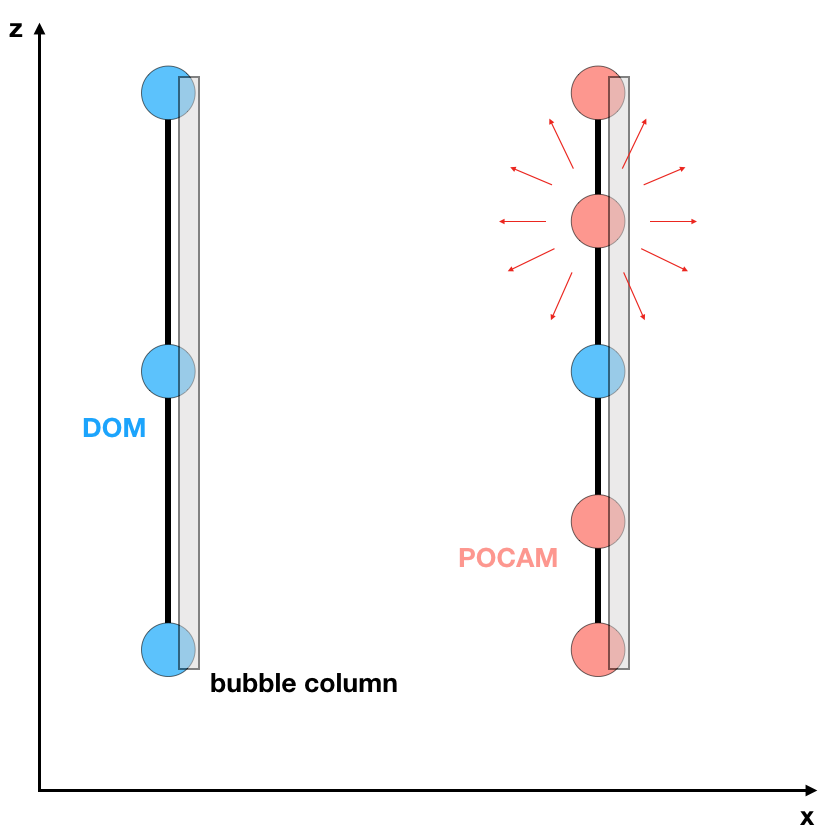
\includegraphics[width=0.8\textwidth]{img/pocamscenario-right}
    \end{column}
  \end{columns}

  \bigskip \her{Example scripts will be at: \url{https://github.com/fiedl/hole-ice-scripts}} \bigskip

  \source{\url{https://github.com/fiedl/hole-ice-talk/releases/tag/v1.5}}
\end{frame}

\subsection{\tobedone Implement missing features}
\begin{frame}{\tobedone Implement missing features}
  \begin{description}
    \item[Ice tilt] Re-implementing ice tilt will be relatively easy after the hole-ice code is ported.
    \item[Direct detection] Direct detection has already been implemented during the original study. But we need a switch to turn it on and off.
    \item[Anisotropy] Instead of re-implementing the old ice-anisotropy model, I'd like to coordinate with Martin Rongen and Dima. Maybe it is possible to implement the new anisotropy model discussed in the previous calibration calls. \url{https://drive.google.com/file/d/1TyqDQgHXSKuHBUC0gLo4xz9RKvxk5dGV/view}
  \end{description}
\end{frame}

\subsection{\tobedone Merge hole-ice code into clsim trunk}
\begin{frame}{\tobedone Merge hole-ice code into clsim trunk}
  \begin{itemize}
    \item When everything works as expected:
    \item[\tobedone] Port hole-ice code to svn trunk of the icecube-simulation framework
    \item[\tobedone] Create a feature branch based on trunk on the svn
    \item[\tobedone] Coordinate with the clsim maintainer, Claudio Kopper, to get it accepted into the framework
  \end{itemize}
\end{frame}
